\documentclass[14pt]{beamer}
\usepackage[utf8]{inputenc}
\usepackage{polski}

\usetheme[height=1cm]{Rochester}
\usecolortheme[RGB={0,156,201}]{structure}
\usefonttheme{professionalfonts}
\setbeamertemplate{navigation symbols}{}

\title{Monady w programowaniu funkcyjnym}
\author{Łukasz Dąbek}

\begin{document}

\begin{frame}[plain]
    \titlepage
\end{frame}

\begin{frame}{Samouczki}
    \begin{center}
        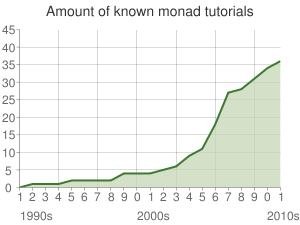
\includegraphics[scale=0.5]{monads-timeline.png}
    \end{center}
\end{frame}

\begin{frame}{Zwięzła definicja}
    \begin{quote}
        A monad is just a monoid in the category of endofuctors,
        what's the problem?
        \vskip5mm
        \hspace*\fill{\small--- Philip Wadler \pause (coż, nie do końca)} 
    \end{quote}
\end{frame}


\begin{frame}{I Ty możesz odkryć monady}
    \begin{itemize}
        \item Standardowa metoda: abstrakcyjne coś $\rightarrow$ zastosowania.
        \pause
        \item Dzisiejsza metoda: zastosowania $\rightarrow$ abstrakcyjne coś.
        \item (Podziękowania dla Dana Piponiego)
    \end{itemize}
\end{frame}

\begin{frame}{Funkcje debugowalne}
    \begin{itemize}
        \item Debugowanie w języku nieczystym jest proste
            (\texttt{printf} w dowolnym miejscu).
        \pause
        \item Jak poradzić sobie w Haskellu?
    \end{itemize}
\end{frame}

\begin{frame}{Funkcje debugowalne}
    \texttt{f, g :: Float -> Float}
    \pause

    \texttt{f x = x * 4}

    \texttt{g x = x + 2}
\end{frame}

\begin{frame}{Funkcje debugowalne}
    \texttt{f', g' :: Float -> (Float, \emph{String})}
    \pause

    \texttt{f' x = (x * 4, "f was called")}

    \texttt{g' x = (x + 2, "g " ++ show x)}
\end{frame}

\begin{frame}{Kompozycja}
    \begin{itemize}
        \item Chcemy prześledzić wykonanie złożenia funkcji \texttt{f'}
            i \texttt{g'}.
        \item Złożenie \texttt{f} i \texttt{g} to \texttt{f . g}.
        \item Jak złożyć \texttt{f'} i \texttt{g'}?
    \end{itemize}
\end{frame}

\begin{frame}[fragile]
\frametitle{Kompozycja}
\begin{verbatim}
let (y, s) = g' x
    (z, t) = f' y in (z, s ++ t)
\end{verbatim}
\end{frame}

\begin{frame}{Kompozycja}
    \begin{itemize}
        \item Nie chcemy pisać tego kodu wielokrotnie.
        \item \texttt{bind f' :: (Float,String) -> (Float,String)}
    \end{itemize}
\end{frame}

\begin{frame}[fragile]
\frametitle{Bind}
\begin{verbatim}
bind :: (Float -> (Float,String))
     -> (Float,String)
     -> (Float,String)
\end{verbatim}
\end{frame}

\begin{frame}[fragile]
\frametitle{Bind}
\begin{verbatim}
bind f (x,s) =
  let (y,t) = f x in (y,s ++ t)
\end{verbatim}
\end{frame}

\begin{frame}[fragile]
\frametitle{(*)}
\begin{verbatim}
(*) :: (Float -> (Float,String))
    -> (Float -> (Float,String))
    -> (Float -> (Float,String))

f * g = \x -> bind g (f x)
\end{verbatim}
\pause

\texttt{f . g = \char`\\x -> g (f x)}
\end{frame}

\begin{frame}{A identyczność?}
    \begin{itemize}
        \item \texttt{id x = x}
        \item Miła własność: \texttt{f . id = id . f = f}.
        \item Co jest odpowiednikiem \texttt{id} w przypadku
            funkcji debugowalnych?
    \end{itemize}
\end{frame}

\begin{frame}{Unit}
    \texttt{unit :: Float -> (Float,String)\\
    unit x = (x,"")}
\end{frame}

\begin{frame}{Unit - przykład dowodu}
    \texttt{(f * unit) x\\
        = bind f (unit x)\\
        = bind f (x, "")\\
        = let (y,s) = f x in (y,""++s)\\
        = let (y,s) = f x in (y, s)\\
        = f x
    }
\end{frame}

\begin{frame}{Kolejna własność kompozycji}
    \begin{itemize}
        \item Kompozycja funkcji jest łączna:
        \item \texttt{f . (g . h) = (f . g) . h}
        \item Spodziewamy się tego również w przypadku funckji debugowalnych.
    \end{itemize}
\end{frame}

\begin{frame}{Łączność (*)}
    \begin{itemize}
        \item \texttt{f * (g * h) = (f * g) * h}
        \pause
        \item Pozostawiamy dowód jako ćwiczenie.
    \end{itemize}
\end{frame}

\begin{frame}{Funkcje niedebugowalne}
    \begin{itemize}
        \item Jak składać funkcje debugowalne ze zwykłymi?
        \item \texttt{f  :: Float -> Float}
        \item \texttt{g' :: Float -> (Float,String)}
        \pause
        \item \texttt{unit . f :: Float -> (Float,String)}
        \item \texttt{unit . f * g'}
    \end{itemize}
\end{frame}

\begin{frame}[fragile]
\frametitle{Lift}
\begin{verbatim}
lift :: (Float -> Float)
     -> (Float -> (Float,String))
lift f = unit . f

lift f * lift g = lift (f . g)
\end{verbatim}
\end{frame}

\begin{frame}{Małe podsumowanie}
    \begin{itemize}
        \item \texttt{type Dbg a = (a,String)}
        \item \texttt{f, g::Float -> Float}
        \item \texttt{f', g'::Float -> Dbg Float}
        \item \texttt{bind::(a -> Dbg b) -> Dbg a -> Dbg b}
        \item \texttt{unit::a -> Dbg a}
    \end{itemize}
\end{frame}

\begin{frame}{Checkpoint}
    \begin{itemize}
        \item Pierwsza monada za nami!
        \item Znana jako \texttt{Writer monad} (patrz: \texttt{Control.Monad.Writer}).
        \item Jeszcze do niej wrócimy.
        \pause
        \item Pytania?
    \end{itemize}
\end{frame}


\begin{frame}{Funkcje wielowartościowe}
    Pierwiastek kwadratowy (sześcienny) z dodatniej liczby rzeczywistej
    jest funkcją jednowartościową.
\end{frame}

\begin{frame}{Funkcje wielowartościowe}
    \texttt{sqrt, cbrt :: Float -> Float}
    \pause

    \texttt{sixthRoot = sqrt . cbrt}
\end{frame}

\begin{frame}{Funkcje wielowartościowe}
    W przypadku liczb zespolonych każda niezerowa liczba ma n pierwiastków
    n-tego stopnia.
\end{frame}

\begin{frame}{Funkcje wielowartościowe}
    \texttt{sqrt', cbrt' :: Complex -> [Complex]}
\end{frame}

\begin{frame}{Kompozycja}
    \begin{itemize}
        \item Chcemy złożyć funkcje \texttt{sqrt'} i \texttt{cbrt'}.
        \item Problem: \texttt{sqrt'} nie przyjmuje listy!
    \end{itemize}
\end{frame}

\begin{frame}{Kompozycja}
    \texttt{sixthRoot x = concatMap sqrt' (cbrt' x)}

    \texttt{concatMap :: (a -> [b]) -> [a] -> [b]\\
    concatMap = concat . map}
\end{frame}

\begin{frame}{Bind}
    \begin{itemize}
        \item \texttt{bind$_d$::(a -> Dbg b) -> Dbg a -> Dbg b}
        \item \texttt{concatMap::(a -> [b]) -> [a] -> [b]}
    \end{itemize}
\end{frame}

\begin{frame}{Monada listowa}
    \begin{itemize}
        \item \texttt{type Mv a = [a]}
        \item \texttt{bind$_m$ = concatMap}
        \item \texttt{unit$_m$ x = [x]}
    \end{itemize}
\end{frame}

\begin{frame}{Monady ogólnie}
    Widzieliśmy przykłady, teraz będzie bardziej abstrakcyjnie.
\end{frame}

\end{document}
